\chapter{The software architecture of WRF}\label{ch:arch}

WRF is about two million lines of Fortran, and its design is what makes a large change such as a GPU port
possible. This chapter describes:
\begin{itemize}
  \item the three layers of the code;
  \item the domain data structure and its index conventions;
  \item the Registry, from which much of the code is generated.
\end{itemize}
All three decide where GPU directives can go and how data reaches the device.

\section{Three layers}

\begin{figure}[ht]
\centering
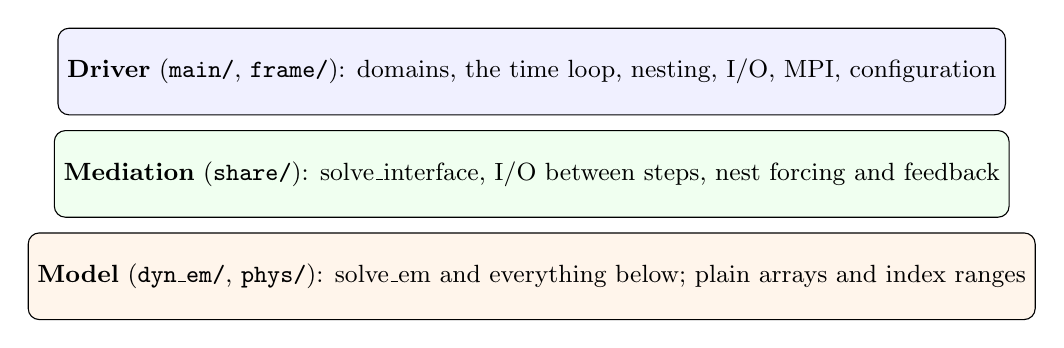
\begin{tikzpicture}[box/.style={draw, rounded corners, minimum width=11cm, minimum height=1.1cm, align=left, font=\small}]
  \node[box, fill=blue!6] (d) at (0,2.6) {\textbf{Driver} (\texttt{main/}, \texttt{frame/}): domains, the time loop, nesting, I/O, MPI, configuration};
  \node[box, fill=green!6] (m) at (0,1.3) {\textbf{Mediation} (\texttt{share/}): solve\_interface, I/O between steps, nest forcing and feedback};
  \node[box, fill=orange!8] (o) at (0,0) {\textbf{Model} (\texttt{dyn\_em/}, \texttt{phys/}): solve\_em and everything below; plain arrays and index ranges};
\end{tikzpicture}
\caption{The three layers of WRF. Only the driver and mediation layers see the domain type as a whole; model-layer
routines receive arrays and dimensions as arguments.}
\label{fig:layers}
\end{figure}

\begin{description}
  \item[Driver layer.] \code{main/wrf.F} calls \code{wrf_init}, \code{wrf_run} and \code{wrf_finalize}
    (\code{main/module_wrf_top.F}). The run is the recursive \src{frame/module_integrate.F}{integrate} of
    \cref{ch:bdy}: one call per domain, advancing it and its nests. This layer owns the domains, the clocks, the I/O
    and the parallel infrastructure.
  \item[Mediation layer.] \code{share/} holds the routines that connect the driver to the model:
    \code{solve_interface}, which calls \code{solve_em} for one domain step, and \code{mediation_integrate.F}, which
    decides before and after each step whether to read boundary data or write history and restart files. It also
    holds nest forcing (\code{mediation_force_domain.F}) and feedback.
  \item[Model layer.] \code{dyn_em/solve_em.F} and everything it calls: the dynamics and, through the physics
    drivers, the schemes in \code{phys/}. Model-layer routines are \emph{tile-callable}: they receive arrays and
    the index ranges of the domain, the memory and the tile, and compute only on the tile.
\end{description}

\begin{portnote}
The layering helps the port in two ways:
\begin{itemize}
  \item the model-layer routines see plain arrays, so a GPU kernel in them needs no knowledge of the domain type;
  \item data movement between host and device can be concentrated at the layer boundaries: the step bracket around
    \code{solve_em}, I/O in the mediation layer, nest forcing.
\end{itemize}
\Cref{ch:port} uses exactly these points.
\end{portnote}

\section{The domain type}

Each domain is a variable of the derived type \code{domain} (\code{frame/module_domain_type.F}). It holds:
\begin{itemize}
  \item every state array of the domain: about 1{,}660 \code{state} entries are declared in
    \code{Registry.EM_COMMON} alone;
  \item the domain's configuration, clocks and alarms;
  \item pointers to its parent, nests and siblings.
\end{itemize}
Domains form a tree rooted at \code{head_grid}. Arrays are allocated for a domain only if they are in use for its
configuration: a scheme's arrays exist only when its \emph{package} is selected. Species of the same kind are
grouped into four-dimensional arrays with a species index:
\begin{itemize}
  \item \code{moist(:,:,:,P_QV)}, \dots;
  \item \code{scalar}, \code{chem}, \code{tracer}.
\end{itemize}
The index constants \code{P_QV}, \code{P_QC}, \dots{} are variables set at startup from the packages in use, not
compile-time constants.

\section{Dimensions}

Every model-layer routine receives four sets of index bounds per direction:
\begin{center}
\begin{tabular}{ll}
\toprule
Bounds & Meaning \\
\midrule
\code{ids:ide}, \code{jds:jde}, \code{kds:kde} & the whole domain (staggered extent) \\
\code{ims:ime}, \code{jms:jme}, \code{kms:kme} & the memory of this process: its patch plus a halo \\
\code{ips:ipe}, \code{jps:jpe}, \code{kps:kpe} & the patch: the part of the domain this MPI process owns \\
\code{its:ite}, \code{jts:jte}, \code{kts:kte} & the tile: the part of the patch one thread computes \\
\bottomrule
\end{tabular}
\end{center}
Arrays are dimensioned by the memory bounds, \code{(ims:ime, kms:kme, jms:jme)}, with $i$ fastest and the vertical
index in the middle. Loops run over the tile, clipped to the domain where a staggered or unstaggered field ends:
\code{MIN(ite, ide-1)} for a mass point.

\section{The Registry}

\code{WRF/Registry/} contains text files that declare, one line per item:
\begin{itemize}
  \item the state arrays;
  \item the temporaries of the solver;
  \item the namelist options;
  \item the packages of each scheme;
  \item the halo exchanges and the I/O streams.
\end{itemize}
A program, \code{tools/registry}, reads them at build time and generates Fortran: declarations, allocation,
I/O calls, communication and nest interpolation (\cref{ch:iobuild}). The line for the $x$-wind is
\begin{lstlisting}[language={}]
state  real  u  ikjb  dyn_em  2  X  i0rhusdf=(bdy_interp:dt)  "U"  "x-wind component"  "m s-1"
\end{lstlisting}
Its fields are:
\begin{itemize}
  \item a state array of type real named \code{u};
  \item dimensions $i$, $k$, $j$ plus boundary arrays (\code{ikjb});
  \item used by the \code{dyn_em} core, with two time levels (\code{u_1}, \code{u_2});
  \item staggered in X;
  \item the I/O and nesting flags \code{i0rhusdf}: input stream 0, restart, history, and the nesting flags (up, smooth,
    down, force), with \code{bdy_interp} as the forcing interpolator;
  \item its name in files, a description and units.
\end{itemize}
Other entry types:
\begin{itemize}
  \item \code{i1} declares a temporary of the solver, an automatic array of \code{solve_em} (for example
    \code{ru_tendf});
  \item \code{rconfig} declares a namelist option;
  \item \code{package} ties a namelist value to the arrays it needs, for example
    \code{package wsm6scheme mp_physics==6 - moist:qv,qc,qr,qi,qs,qg;...};
  \item \code{halo} and \code{period} declare communication;
  \item \code{xpose} declares a transpose for the polar filters.
\end{itemize}

\begin{portnote}
The Registry is the single source of truth for which fields exist, so the port generates its data movement from it,
as WRF generates its own code:
\begin{itemize}
  \item \code{tools/gen_allocs.c} gains one call per array that makes it resident on the device when it is allocated;
  \item a new generator, \code{tools/gen_gpu.c}, writes the update lists of every field, of the boundary fields, and
    of the fields that nest forcing reads and writes;
  \item the solver temporaries (\code{i1}) become views into one persistent pool on the device.
\end{itemize}
No list of fields is maintained by hand (\cref{ch:port}).
\end{portnote}

\section{The step from the top}

\begin{algorithm}[ht]
\caption{From \code{wrf.exe} to one model step (one-way nest, simplified).}
\label{alg:top}
\begin{algorithmic}[1]
\State \code{wrf_init}: read the namelist, allocate \code{head_grid}, read initial data (\code{med_initialdata_input}), initialize (\code{start_domain})
\State \code{integrate(head_grid)}:
\While{the domain's clock is before its stop time}
  \State open nests whose start time has come (\code{med_nest_initial})
  \State \code{med_before_solve_io}: read boundary data, write history and restart if due
  \State \code{solve_interface} $\to$ \code{solve_em} (\cref{alg:solve-em})
  \State \code{med_after_solve_io}
  \For{each nest}
    \State \code{med_nest_force}; \code{integrate(nest)} for its steps; \code{med_nest_feedback}
  \EndFor
\EndWhile
\State \code{wrf_finalize}: last output, deallocation
\end{algorithmic}
\end{algorithm}
